\section{Experimente}
\label{sec:experimente}
In diesem Paper werden die Experimente aus \cite{rstensorflow2017} nachgestellt, um so eine Validierung der dortigen Ergebnisse zu ermöglichen. Damit die Resultate vergleichbar sind, werden die Experimente rekonstruiert. Diese Rekonstruktion wird in \ref{subsec:rekonstruktion} genauer beschrieben. Zusätzlich zu den in \cite{rstensorflow2017} verwendeten Metriken, wie beispielsweise die Ausführungszeit, werden in dieser Arbeit weitere mögliche Metriken in Abschnitt \ref{subsec:metriken} für eine Anwendung beim Vergleich zwischen Eigen und RenderScript diskutiert. Ebenso wird in Abschnitt  \ref{subsec:anpassungentf} erläutert, welche Änderungen am Quellcode von RSTensorFlow durchgeführt wurden. Für diese Modifikationen wurde ein neuer Fork \cite{rstfengelmi} vom RSTensorFlow-Repository auf GitHub erstellt. Hier wurden im Branch \textit{RenderScript} nicht nur die Code-Änderungen veröffentlicht, sondern auch die Ergebnisse der in \ref{subsec:experimentauswertung} dargestellten Auswertungen. 
\\
Während in \cite{rstensorflow2017} zwei Nexus-Geräte für die Durchführung der Experimente genutzt wurde, werden in dieser Arbeit zwei Samsung-Smartphones verwendet. Die Tabelle \ref{tbl:hardware} stellt die genaueren Spezifikationen dieser Hardware dar. 
\renewcommand{\arraystretch}{1.5}
\begin{table}[!ht]
	\begin{center}
		\begin{tabular}{c||p{3.0cm}|p{3.1cm}}
			\textbf{Modell} & Samsung J5 & Samsung S7 \\
			\hline
			\textbf{Android OS} & 6.0 & 6.0 \\
			\hline
			\textbf{CPU} & 4x1,2 GHz & 4x2,3 GHz und 4x1,6 GHz \\
			\hline
			\textbf{GPU} & Adreno 306 & Mali-T880 MP12 \\ 
			\hline
			\textbf{RAM} & 1,5 GB & 4 GB \\
		\end{tabular}
	\end{center}
	\caption{Ein Auszug aus der Hardware-Spezifikation nach \url{https://www.gsmarena.com} für die gewählten Smartphone-Modelle für die Experimente. }
	\label{tbl:hardware}
\end{table}

\subsection{Rekonstruktion}
\label{subsec:rekonstruktion}
Damit die in dieser Arbeit durchgeführten Experimente mit denen aus \cite{rstensorflow2017} vergleichbar sind, wird versucht diese zu rekonstruieren. In \cite{rstensorflow2017} liegt der Fokus für die Bewertung der RenderScript-Implementierung auf den beiden Operationen matmul und conv2D. Hierfür wurden die Metriken
\begin{itemize}
	\item CPU-Last und
	\item Ausführungszeit
\end{itemize}
betrachtet. 
\\
Für die Messung der Auslastung der CPU wurde die App \textit{Trepn Profiler} eingesetzt. Für die Messungen der Ausführungszeit wurde der Quellcode angepasst und ein Block zur Zeitmessung um die Anweisung für die jeweilige Operation gesetzt. Das Ergebnis wird dann auf einen Ausgabestrom gegeben, auf welchem mit dem \textit{ADB}-Tool zugegriffen werden kann. Dies kann in den beiden Quellcode-Dateien 
\begin{itemize}
	\item conv\_ops.cc und
	\item matmul\_op.cc
\end{itemize}
überprüft werden. Jedoch sind bei den Auswertungen der Experimente in \cite{rstensorflow2017} Multiplikationen mit quadratischen Matrizen dargestellt. Das Google Inception Model, welches von der TF Classify App verwendet wird, nutzt jedoch keine quadratischen Matrizen. In der Auswertung für die Convolution-Operation werden Filterzahlen aufgeführt, welche ebenfalls nicht im Google Inception Model für diese Operation definiert sind. Daher wird vermutet, dass für die Experimente in \cite{rstensorflow2017} eine separate App genutzt wurde. In dieser Arbeit wird direkt auf der TF Classify App aufgesetzt. Somit ändern sich die Größen der Matrizen und die Anzahl der Filter. Die Vergleichbarkeit zu den Experimenten aus \cite{rstensorflow2017} bleibt trotzdem bestehen, da es sich hier um variable Größen handelt und für den Vergleich zwischen Eigen und RenderScript weiterhin die gleiche Metrik verwendet wird. 

\subsection{Metriken}
\label{subsec:metriken}
In \cite{rstensorflow2017} werden als Metriken für den Vergleich zwischen Eigen und RenderScript die Ausführungszeit und Auslastung der CPU bei der Ausführung einer Operation betrachtet. Häufig werden weitere Metriken bei der Bewertung von Bibliothek für mobile Geräte wie Eigen oder RenderScript herangezogen. In \cite{deepmon2017} wird u.a. auch der Stromverbrauch gemessen. Diese Metrik ist gerade bei mobilen Geräten mit der limitierten Akkulaufzeit von großer Bedeutung. Diese Metrik wird in dieser Arbeit jedoch nicht genutzt. Der Fokus liegt auf Metriken, um die Performance beurteilen zu können. 
\\
Über die Trepn Profiler App lassen sich viele Kenngrößen der Performance auf mobilen Geräten messen. So kann nicht nur die Last der CPU im Allgemeinen, sondern sogar jedes einzelnes Kerns genau aufgezeichnet werden. Im Rahmen des Experimentes ist dieser Detailgrad nicht nötig, weshalb nur die gesamte CPU-Auslastung interessant ist. Die Autoren von RSTensorFlow vermuteten bei Ihrer Auswertung der Experimente einen Zusammenhang zwischen der schlechteren Performance von RenderScript und der Nutzung des Arbeitsspeichers. Daher wird diese Ressource über den Trepn Profiler aufgezeichnet. Eine weitere, interessante Metrik ist die Auslastung der GPU. Durch das Aufzeichnen dieser Kenngröße ist es möglich festzustellen, ob RenderScript tatsächlich in der Lage ist die Rechenressourcen mobiler Geräte zu nutzen. Diese Größe kann von der Trepn Profiler App nur für das Samsung J5 mitgeschnitten werden. Die GPU-Last ist für das Samsung S7 durch den Trepn Profiler leider nicht aufzuzeichnen, da diese App die in dem Gerät verbaute GPU nicht unterstützt. Die Verwendung einer alternativen Anwendung ist keine Option, da für das Experiment die gleiche Anwendung wie in der Referenzarbeit zu nutzen ist. 
\\
Über die Android Debug Bridge können die Ausführungszeiten von Operationen aufgezeichnet werden. Für die Matrixmultiplikation sind jedoch auch Informationen bezüglich der Größe der beteiligten Matrizen von Bedeutung. Das Gleiche gilt für die Convolution-Operation. Hier sind Informationen wie beispielsweise die Größe der Tensoren oder die Größe des Strides interessant. Die Anzahl der verwendeten Filter für die Convolution-Operation entspricht genaue der Tiefe des Output-Tensors, weshalb für die Filterzahl keinerlei weitere Informationen ermittelt werden müssen. Die für das Aufzeichnen dieser Daten nötigen Anpassungen am Quellcode werden in \ref{subsec:anpassungentf} näher erläutert. 

\subsection{Anpassungen von RSTensorFlow}
\label{subsec:anpassungentf}
Im Abschnitt \ref{subsec:metriken} wurde Notwendigkeit von Anpassungen des Quellcodes von RSTensorFlow dargestellt. Diese Änderungen werden in den C++-Dateien 
\begin{itemize}
	\item conv\_ops.cc und
	\item matmul\_op.cc
\end{itemize}
direkt im Kernel von TensorFlow vorgenommen. RSTensorFlow hat in beiden Klassen bereits einen einfachen Mechanismus zur Ermittlung der Ausführungszeit innerhalb der Methode
\begin{lstlisting}
    void Compute(OpKernelContext* ctx)
\end{lstlisting}
implementiert. Die Ausgabe der Zeit wird mit einem \textit{stringstream} umgesetzt, welcher innerhalb der Android-App den Stream für das Logging verwendet. Somit lassen sich die Informationen aus dem Kernel wie einfache Log-Ausgaben mit dem ADB-Tool abgreifen. Für die Android-Apps von TensorFlow entspricht dies dem Befehl: 
\begin{lstlisting}
    adb logcat -s TF\_ANDROID\_LOG
\end{lstlisting}
Die Ausgabe wird nun für die Matrixmultiplikation um Form der beiden Matrizen und der Ergebnis-Matrix erweitert. Bei der Convolution-Operation wird die Ausgabe des String-Streams um die Form des Eingabe-, Filter- und Ausgabe-Tensors sowie des zu verwendenden Strides und das sog. Zero-Padding erweitert. Für das einfache Wechseln zwischen der Eigen- und RenderScript-Implementierung wird außerdem die Präprozessor-Anweisung 
\begin{lstlisting}
    #define USE_RENDERSCRIPT
\end{lstlisting}
festgelegt. Ist diese definiert, so wird beim bauen der Android-Apps die RenderScript-Implementierung verwendet. Damit stattdessen die Eigen-Bibliothek genutzt wird muss dieses Flag lediglich auskommentiert werden. Die Steuerung des Wechsels über die Oberfläche der fertigen Android-App wäre eine mögliche Erweiterung. 
\\
Die hier beschriebenen Änderungen sind im GitHub-Repository \cite{rstfengelmi} unter dem Branch \textit{RenderScript} einsehbar. 

\subsection{Aufbau und Durchführung}
\label{subsec:aufbauexperiment}
Für das Aufzeichnen der Daten per ADB wird das Smartphone mit einem USB-Kabel an einen Laptop angeschlossen. Auf diesem wird dann das ADB-Logging gestartet. Die Trepn Profiler App wiederum speichert die Daten in eine CSV-Datei auf den Speicher des Smartphones. 
\\
Zunächst werden in der Trepn Profiler App die nötigen Einstellungen, wie beispielsweise die aufzuzeichnenden Metriken, festgelegt. Vor dem Start des Experiments wird das Smartphone vollständig geladen, alle Programme geschlossen und das WLAN deaktiviert. Sobald das mobile Gerät am Laptop angeschlossen wurde, wird mit 
\begin{lstlisting}
    adb logcat -c
\end{lstlisting}
der logcat-Buffer geleert und anschließend das ADB-Logging gestartet. Die Trepn Profiler App kann den Arbeitsspeicher nur für das gesamte System ermitteln. Um nun den durch die TF Classify App verbrauchten Speicher zu bestimmen, wird zunächst das Logging durch Trepn Profiler gestartet und mit dem Starten der TF Classify App wenige Sekunden gewartet. In diesen ersten Momenten wird der Arbeitsspeicher des Systems \glqq im Ruhezustand\grqq~ermittelt und kann zur Berechnung des durch die TF Classify App verbrauchten Arbeitsspeichers verwendet werden. Nach ca. 6 Minuten wird das sog. Profiling durch Trepn Profiler und das ADB Logging gestoppt. 
\\
Diese Routine wird für beide in der Tabelle \ref{tbl:hardware} aufgeführten Geräte mit RSTensorFlow jeweils mit Eigen- und RenderScript-Unterstützung durchgeführt. 

\subsection{Auswertung}
\label{subsec:experimentauswertung}
Für eine einfachere Auswertung werden die aufgezeichneten Daten zunächst aufbereitet. Während die CSV-Dateien der Trepn Profiler App manuell vorbereitet werden, wird für die durch das ADB-Logging aufgezeichneten Daten ein Python-Skript genutzt. Die aufbereiteten Daten werden mit einem R-Skript visualisiert. 
\\
\subsubsection{Matrixmultiplikation}
\label{subsubsec:matmulauswertung}
In Abbildung \ref{fig:matrizengroesse} sind die gemittelten Zeiten in Millisekunden für die von TF Classify durchgeführten beiden Arten der Matrizenmultiplikation zu sehen. Auf dem Samsung S7 benötigte RenderScript ungefähr doppelt so lange für beide Arten von Multiplikation. Für das Samsung J5 fällt diese Spanne wieder um einiges größer aus. Bei einer Matrixmultiplikation der Form
\begin{center}
	$R^{1 \times 1024} \times R^{1024 \times 1008} \rightarrow R^{1 \times 1008}$
\end{center}
benötigt Eigen nur etwa ein Drittel der Zeit im Vergleich zu RenderScript. Für eine Matrixmultiplikation der Form 
\begin{center}
	$R^{1 \times 2048} \times R^{2048 \times 1024} \rightarrow R^{1 \times 1024}$
\end{center}
ist RenderScript schon fast 10 Mal langsamer als Eigen. 
\begin{figure}[!t]
	\centering
	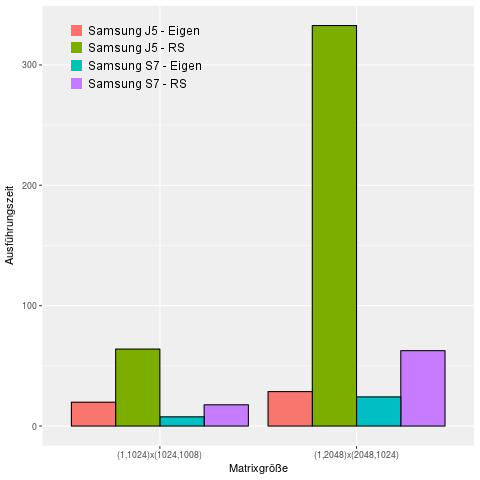
\includegraphics[width=3.0in]{images/aa-paper-matrizengroesse-legende.jpg}
	\caption{Die Ausführungszeiten in Millisekunden der von TF Classify durchgeführten Matrizenmultiplikationen. }
	\label{fig:matrizengroesse}
\end{figure}
Dieses Ergebnis widerspricht teilweise den Resultaten aus \cite{rstensorflow2017} bezüglich der Zeiten für die Matrixmultiplikation. Hier wurde, zumindest für das Nexus 5X, eine Performance-Steigerung festgestellt. Allerdings war RenderScript auf diesem Smartphone nach \cite{rstensorflow2017} in der Lage die GPU zu nutzen. Dies würde implizieren, dass RenderScript sowohl auf dem Samsung J5 als auch auf dem Samsung S7 die GPU nicht verwenden konnte. Bei Betrachtung der CPU-Last für das J5 ist festzustellen, dass die CPU unter der Verwendung von RenderScript durchgehend fast 100\% ausgelastet war. Die Eigen-Variante hingegen lastete hier die CPU im Schnitt mit 80\% aus. Auf dem Samsung S7 wiederum lastet Eigen die CPU stärker aus als RenderScript. Dies könnte trotz der längeren Laufzeit auf die Nutzung der GPU durch RenderScript hindeuten, wobei dies aufgrund der fehlenden Messwerte von der GPU nicht mit Sicherheit behauptet werden kann. 

\subsubsection{Convolution}
\label{subsubsec:convauswertung}
Die visualisierten Daten der Convolution-Operation unterstützen die in \ref{subsubsec:matmulauswertung} getroffene Schlussfolgerung, dass RenderScript keine GPU auf dem Samsung J5 nutzen kann. Für dieses Gerät wurden im Vergleich zu Eigen deutlich höhere Ausführungszeiten bei der Nutzung von RenderScript gemessen.  Dabei steigt die Zeit allerdings nicht konstant mit der Anzahl verwendeter Filter. Dies liegt darin begründet, dass die Komplexität einer Convolution-Operation nicht nur von der Anzahl anzuwendender Filter abhängt. Die Größe des Input- und Filter-Tensors sowie die Größe des Strides und das Zero-Paddings sind hierfür ebenfalls relevante Parameter. Beim Samsung S7 hingegen hat RenderScript überraschenderweise und entgegen der Ergebnisse in \cite{rstensorflow2017} die Convolution-Operationen oftmals schneller durchgeführt als Eigen. Ab 64 Filtern ist RenderScript ungefähr doppelt so schnell wie die Eigen-Bibliothek. In \cite{rstensorflow2017} wurde die schlechtere Performance von RenderScript bei der Convolution-Operation mit einem Overhead bei der Reservierung von Arbeitsspeicher versucht zu begründen. 
\begin{figure}[!t]
	\centering
	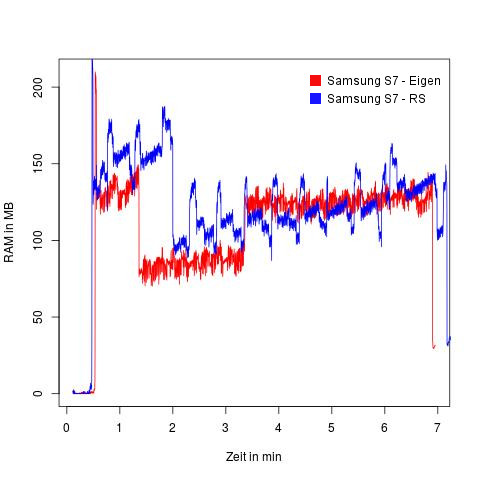
\includegraphics[width=3.0in]{images/s7Trepn-eigen-rs-memory-app-legende.jpg}
	\caption{Ein Vergleich des benötigten Arbeitsspeichers von TF Classify zwischen der RenderScript- und Eigen-Implementierung.}
	\label{fig:s7ram}
\end{figure}
Wie in Abbildung \ref{fig:s7ram} zu sehen ist, wird bei RenderScript häufiger eine etwas größere Menge Speicherplatz reserviert. Da die Convolution-Operation bei RenderScript trotzdem schneller durchgeführt wurde, wird dies vermutlich keinen signifikanten Einfluss auf die Ausführungszeit haben. Eine mögliche Erklärung für den Performance-Unterschied kann auch die Nutzung der GPU nicht sein, da in \cite{rstensorflow2017} RenderScript auf dem Nexus 5x diese Rechenressource nutzt und dennoch eine schlechtere Performance als Eigen erzielt. Ein Unterschied bei der Hardware zwischen dem Nexus 5X und dem Samsung S7 ist die Anzahl und Frequenz der CPU-Kerne. Bei der Convolution-Operation einzelnen Ebenen in der Tiefe des Filter-Tensors unabhängig voneinander auf den Eingabe-Tensor angewandt werden können, sind diese Operationen gut parallelisierbar. Daher liegt die Vermutung nahe, dass RenderScript diese Parallelisierung besser nutzen kann als Eigen. 
\begin{figure}[!t]
	\centering
	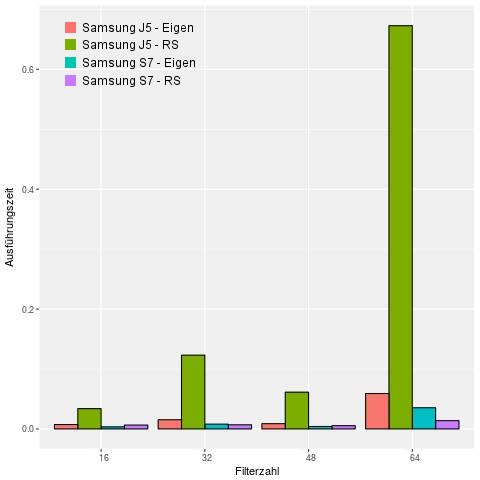
\includegraphics[width=3.0in]{images/aa-paper-filteranzahl-1-legende.jpg}
	\caption{Die Ausführungszeiten in Millisekunden der von TF Classify durchgeführten Convolution-Operation für 16 bis 64 anzuwendende Filter. }
	\label{fig:filterzahl1}
\end{figure}

\begin{figure}[!t]
	\centering
	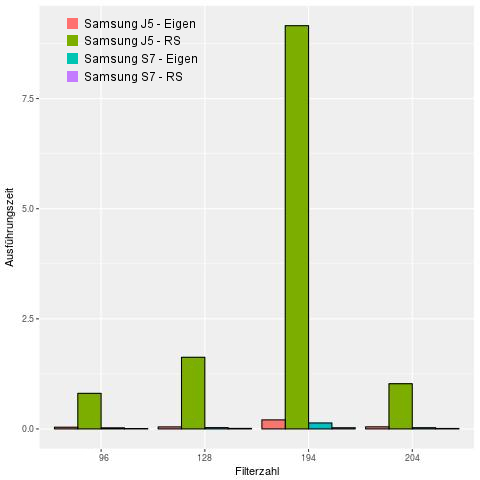
\includegraphics[width=3.0in]{images/aa-paper-filteranzahl-2-legende.jpg}
	\caption{Die Ausführungszeiten in Millisekunden der von TF Classify durchgeführten Convolution-Operation für 96 bis 204 anzuwendende Filter. }
	\label{fig:filterzahl2}
\end{figure}

\subsubsection{Inference-Pfad}
\label{subsubsec:inferencepfad}
Bei der Gesamtdauer eines einzelnen Inference-Pfades fallen für beide mobile Geräte deutliche Unterschiede zwischen der Eigen- und RenderScript-Variante auf. Beim Samsung S7 dauert ein Pfad mit der Eigen-Implementierung im Schnitt 0,4s. Die Variante mit RenderScript hingegen führt einen Pfad zwischen 0,8s und knapp 1,2s aus und benötigt damit mindestens zweimal so lange wie Eigen. Für das Samsung J5 fällt dieser Unterschied wesentlich ausgeprägter. Während Eigen einen Pfad im Durchschnitt mit 1s abarbeitet, ist die RenderScript-Variante mit ca. 15s um das 15-fache langsamer. Dies wirkte sich auch auf die Anzahl der durchlaufenen Pfade während des Experiments aus. Beim S7 durchlief die Variante mit Eigen knapp 800 Pfad-Iterationen und mit RenderScript nur knapp die Hälfte. Dieser Sachverhalt wird in Abbildung \ref{fig:s7pfade} besonders deutlich. 
\begin{figure}[!t]
	\centering
	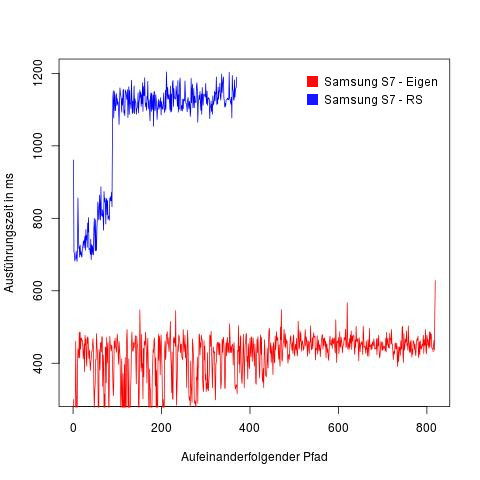
\includegraphics[width=3.0in]{images/s7ADB-eigen-rs-path-legende.jpg}
	\caption{Die Anzahl der durchlaufenen Pfade ist bei der RenderScript-Variante um ca. die Hälfte geringer als bei der Berechnung mit Eigen. }
	\label{fig:s7pfade}
\end{figure}
Demzufolge muss die Verwendung von RenderScript auch indirekte, negative Auswirkungen auf den Inference-Pfad haben. 

